\documentclass[11pt, a4paper]{article}
\usepackage[paper=a4paper, left=1.5cm, right=1.5cm, bottom=1.5cm, top=1.5cm]{geometry}

\usepackage[utf8]{inputenc}
\usepackage[T1]{fontenc}
\usepackage[spanish]{babel}
\usepackage[section]{placeins}
\usepackage{caratula/caratula}
\usepackage{listings}
\usepackage{algorithm}
\usepackage{graphicx}

\parskip = 8pt

\begin{document}

\titulo{Trabajo Práctico}
\fecha{2 de Julio de 2014}
\materia{Teoría de lenguajes}
% \grupo{Grupo 11}
\integrante{Axel Iglesias}{79/10}{axeligl@gmail.com}
\integrante{Agustin Martínez Suñé}{630/11}{agusmartinez.92@gmail.com}
\integrante{Nahuel Lascano}{476/11}{laski.nahuel@gmail.com}
%Carátula

\maketitle
\newpage
Índice
\tableofcontents
\newpage

\section{Introducción}
El objetivo del Trabajo Práctico es crear un lenguaje de programación imperativo que permita definir funciones que serán evaluadas y nos permitirán traficar curvas paramédicas en el plano. 

Para esto, tuvimos que decidir e implementar los siguientes puntos:
\begin{itemize}
\item La gramática que vamos a usar para la implementación
\item El analizador léxico que recibe el código fuente
\item El parser que toma los tokens y verifica que coincida con la gramática
\item El Abstract Syntax Tree que permite representar las funciones del código fuente
\end{itemize}
Para la implementación decidimos utilizar BISON y C++ y utilizamos como referencia la documentación de BISON y el blog que fue recomendado.


\section{Decisiones}
\subsection{BISON}
Como se nombró en la introducción, para la implementación del parser decidimos usar BISON. Esto se debe a la documentación que encontramos para desarrollar el parser y a la aparente sencillez para usarlo.

\subsection{Comentarios}
Con respecto al uso de comentarios en el código fuente, para la primer entrega decidimos usar el comando \textit{sed} para eliminarlos. Esta decisión fue más que nada por ignorancia de cómo implementarlo en BISON. 

Para esta segunda entrega, el lexer se encarga de detectar los comentarios.


\subsection{Curiosidades}
Un detalle que no pudimos confirmar su procedencia, es el error de redondeo que causa nuestra implementación.

En un comienzo, creímos que se debía al uso de Int's en vez de Float's, pero finalmente vimos que no era esa la razón. También creímos que podía ser la precisión de PI, pero \textit{bspline} no utiliza PI.

No logramos encontrar una explicación acorde para este problema.

\section{Resultados}
Para probar la funcionalidad de nuestro parser primogénito creamos los siguientes tests que abarcan las funcionalidades provistas por el lenguaje.

\subsection{Test de funcionalidades básicas}
	El código se encuentra en testsPropios/testBueno1.cod
	\lstinputlisting{testsPropios/testBueno1.cod}
	Salida:
	\lstinputlisting{testsPropios/salidaTest1.out}
\subsection{Test de más funcionalidades}
	El código se encuentra en testsPropios/testBueno2.cod
	\lstinputlisting{testsPropios/testBueno2.cod}
	Salida:
	\lstinputlisting{testsPropios/salidaTest2.out}
	
Ambos tests dan el siguiente gráfico, como era esperado:

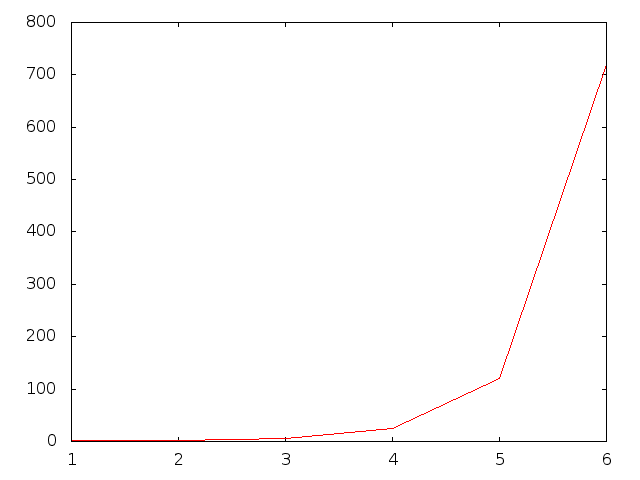
\includegraphics[width=0.60\textwidth,height=0.60\textheight,keepaspectratio]{testsPropios/graficoTest1.png}
\subsection{Tests de desambiguación}
	El código se encuentra en testsPropios/testBueno3.cod
	\lstinputlisting{testsPropios/testBueno3.cod}
	Salida:
	\lstinputlisting{testsPropios/salidaTest3.out}
	
	
	
	En este ejemplo vemos cómo resolvimos el problema de la desambiguación de los ifthenelse anidados. Nuestro enfoque es el mismo que el útilizado en lenguajes de programación conocidos como C. Podemos ver un ejemplo con el siguiente código:
		\lstinputlisting{testsPropios/pruebaIfThenElse.c}
	

\section{Gramática}
El esquelto para hacer la gramática\footnote{implementada en parser.y} fue tomado de la página citada en la presentación\footnote{http://gnuu.org/2009/09/18/writing-your-own-toy-compiler/}. Sobre este esqueleto armamos nuestra gramática, que tiene varios puntos de diferencia con la que muestran de ejemplo en ese sitio.

Nuestra gramática parte de un símbolo incial $programa$ que a su vez se divide en una lista de $funciones$ y una instrucción de $ploteo$.

Una función consiste en la palabra 'function' (representada por el token terminal TFUNC), un $nombre$ (que no es más que un terminal que matchea con strings no empezados por números), una lista de $argumentos$ (lista de $nombre$s separadas por comas) entre paréntesis y un $bloque$ de código.

Un $bloque$ es una lista (quizás vacía) de sentencias encerradas entre llaves o una única sentencia.

Una $sentencia$ puede ser una $asignacion$ (un $nombre$, un símbolo de $=$ y una $expresión$), una sentencia $ifthenelse$, un $while$ (que a su vez tiene una $condicion$ y otro $bloque$) o un $return$ (que lleva a su lado una $expresion$).

El caso del $ifthenelse$ requiere un análisis específico. Un $ifthenelse$ puede tener o no tener 'else', lo cual nos trae una ambiguedad a la hora de parsear cadenas del estilo (intencionalmente sin indentar):
\begin{verbatim}
if cond1 then
if cond2 then
codigo1
else
codigo2
\end{verbatim}
que se refleja en el parser en un conflicto shift/reduce (cuando termina el codigo1 y viene un else puede tanto consumir el else y shiftear como reducir lo que ya tiene).
Para resolverlo, nos basamos en el comportamiento de C en este caso (hacer shift, es decir, que el código se lea como
\begin{verbatim}
if cond1 then
  if cond2 then
    codigo1
  else
    codigo2
\end{verbatim}
) y como Bison por defecto elije hacer siempre shift lo dejamos así.

Una $expresion$ puede ser un $numero$ (entero, double o $\pi$), una $llamada_funcion$ (el nombre de una función con más $expresiones$ entre paréntesis como argumentos) u operaciones aritméticas entre expresiones. Para salvar las ambiguedades propias de esta parte de la gramática le indicamos a Bison la precedencia de los operadores\footnote{basándonos en el código de ejemplo de http://www-h.eng.cam.ac.uk/help/tpl/languages/flexbison/}.

Una $condicion$ puede ser una comparación entre dos $expresion$es u otras condiciones con operadores lógicos.

Por último, la instrucción $ploteo$ consiste en dos $llamada_funcion$ con un $nombre$ de variable y tres $expresion$es que reflejan el inicio, el paso y el final.

La gramática se complementa con un archivo\footnote{tokens.l} con directivas para el tokenizador, que le permite convertir símbolos terminales en los tokens que usamos, ignora saltos de línea y maneja números enteros, floats y cadenas arbitrarias (como los nombres de variables).

Entre los problemas que encontramos hubo uno que no pudimos resolver: no logramos armar la expresión regular para que el tokenizador ignore los comentarios multilínea. Es por esto que para pasar los tests los archivos con comentarios debe ser en primer lugar pasados por un script hecho en bash que los borra.

\section{Respuestas}
\subsection{1er Pregunta}

Para verificar estáticamente que las condiciones de los if y los while sean booleanos se puede utilizar, en la gramática, un no terminal que represente únicamente operaciones booleanas (por ej comparación). De esta forma la gramática se asegura de que las condiciones sean booleanas y al momento de parsear el código se verifica el cumplimiento de ese requisito. De hecho, es así como lo implementamos nosotros.

En los lenguajes de programación tipados probablemente la gramática permita que las condiciones de los if no sean únicamente booleanos pero se verifica a la hora del chequeo de tipos (ya sea estático o dinámico).

\subsection{2da Pregunta} El uso del ; en la gramática de C permite desambiguar código. Veámoslo con un ejemplo:

\lstinputlisting{testsPropios/pruebaPuntoYComa.c}

Este es el código de un ejemplo básico de C. Lo interesante es que, a diferencia de nuestro lenguaje, nos permite poner expresiones como si fueran instrucciones. Las llamadas a funciones en C/C++ son sentencias, a diferencia de nuestro lenguaje donde ninguna funcion tienen efectos secundarios. 

Es por esto que si quitamos los ; del código de ejemplo nos queda una ambigüedad.

\subsection{3ra pregunta}
El orden de definición de las funciones solo importa si queremos verificar, en tiempo de parseo, que las llamadas a función invoquen a una función. Esto se debe a que, al encontrarnos con una llamada a función, solo conoceríamos las funciones que ya parseamos hasta ese momento. Una posible solución es hacer el parsing en dos pasadas, una para reconocer (y guardar en memoria) todos los nombres de función y otra para generar el arbol sintáctico. En nuestro caso, para resolver el problema, no hizo falta este enfoque, ya que verificamos en tiempo de ejecución que las llamadas a función invoquen a funciones válidas.
Por otro lado, para soportar recursión se necesita tener un stack de variables locales por cada llamada a función, lo que permite que dos llamadas a la misma función incluso aunque estén anidadas sean independientes y tengan el comportamiento esperado. Es así como nosotros lo implementamos y por eso nuestro lenguaje soporta recursión.

\section{Manual}
Modo de uso:
\begin{verbatim}
make clean && make
cat archivodetest.cod | ./borracomentarios.sed | ./parser | ./graficador.sh 
\end{verbatim} 

\section{Conclusiones}
Como primer conclusi�n general podemos afirmar que el lenguaje propuesto por la c�tedra es LR1, ya que pudimos construir un parser LR1 que lo reconoce. Adem�s podemos decir que, a pesar de su simpleza, es un lenguaje potente que no solo permite el uso de las cl�sicas estructuras de control de flujo sino que tambi�n, como hemos visto, permite definir funciones de manera recursiva.
Por otro lado el desarrollo de la implementaci�n de este lenguaje de programaci�n nos permiti� terminar de comprender las diferentes etapas que son inherentes a cualquier compilador o int�rprete, desde el reconocimiento de la cadena de entrada y la generaci�n del arbol sint�ctico, hasta etapa de dar sem�ntica a este. 

En ese sentido un punto interesante a remarcar es la relativa independencia de estas etapas. Por ejemplo, si en lugar de interpretar el codigo, simularlo y generar una salida apta para graficar quisieramos traducir las funciones a codigo m�quina para generar un binario ejecutable s�lo deber�amos modificar, en principio, el c�digo que se encarga de manejar el �rbol sint�ctico una vez construido.

\end{document}
